\subsubsection{\bf Overlapping Analysis (RQ5)}

\begin{figure}
	\centering
	\begin{subfigure}{0.235\textwidth}
		\centering
		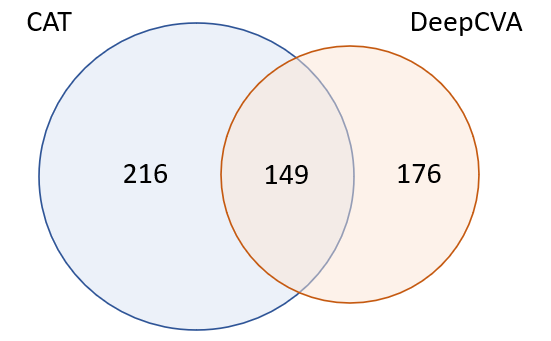
\includegraphics[width=1.65in]{graphs/Overlap-1.png}
		\vspace{-16pt}
		\caption{C Dataset}
		\label{RQ3-result-1}
	\end{subfigure}
	\begin{subfigure}{0.235\textwidth}
		\centering
		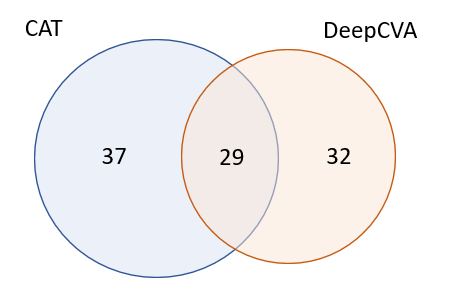
\includegraphics[width=1.65in]{graphs/Overlap-2.png}
		\vspace{-16pt}
		\caption{Java Dataset}
		\label{RQ3-result-2}
	\end{subfigure}
	\vspace{-6pt}
	\caption{Overlapping Analysis}
	\label{RQ3-result}
\end{figure}

Fig.~\ref{RQ3-result} shows the overlaps between the results from
{\tool} and DeepCVA. As seen, on the C dataset, {\tool} correctly
classified 216 commits (regarding all classes for VATs) that were
misclassified by DeepCVA. In contrast, DeepCVA correctly classified
176 commits that were misclassified by {\tool}. Both {\tool} and
DeepCVA correctly classified 149 commits. Moreover, on the Java
dataset, {\tool} can correctly classify 37 Java commits that were
misclassified by DeepCVA. In contrast, DeepCVA can correctly classify
32 Java commits that were misclassified by {\tool}. Both {\tool} and
DeepCVA correctly classified 29 Java commits. Note that the C dataset
(BigVul) is larger than the Java dataset (CVAD). BigVul has 7,851
commits with 785 commits for testing, while CVAD has 1,229 commits
with 123 commits for testing. Thus, the numbers in
Figs~\ref{RQ3-result-1} and~\ref{RQ3-result-2} are much different.
%Tien
%The rationale for choosing the CVAD dataset has two folds. First, we
%aim to compare {\tool} with DeepCVA, which used that dataset in their
%work. Second, we aim to evaluate {\tool} on Java vulnerabilities.


%Figure~\ref{RQ3-result} shows the results of overlapping analysis between {\tool} and DeepCVA on both C and Java datasets on average. On C dataset, {\tool} can correctly classify 2.1K+ C commits but missed by DeepCVA. DeepCVA can correctly classify 1.7K+ C commits but missed by {\tool}. Both {\tool} and DeepCVA can correctly classify 1.5K+ C commits. On Java dataset, {\tool} can correctly classify 37 Java commits but missed by DeepCVA. DeepCVA can correctly classify 32 Java commits but missed by {\tool}. Both {\tool} and DeepCVA can correctly classify 29 Java commits. On both datasets, {\tool} can correctly classify more commits than DeepCVA.



